
\section{Ansatz und Grundgedanken der Implementierung des Architekturteils}
\subsection{Allgemeine Idee}
In der Übersetzungsphase wird jeder Ausdruck (ein Befehl) des Quelltextes durch den Parser eingelesen. Ziel ist es, einen Syntaxbaum zu erstellen, der den Ausdruck in einer Form darstellt, die die geladene Architektur verarbeiten kann. Daraufhin werden die Ausdrücke der Reihe nach als assemblierte Form in den nicht-modifizierbaren Code-Teil des Speichers geschrieben.

\subsubsection{Erzeugung des Syntaxbaumes über das Abstract Factory Pattern}
Die Schnittstelle zum Parser soll so allgemein wie möglich gehalten werden, um Parser und Architekturen austauschen zu können. Die Erzeugung der Knoten für diesen Syntaxbaum wird transparent über eine bzw. mehrere (für jeden Knotentyp eine) Factory(s) geregelt.

Teil der Schnittstelle sind hierbei die abstrakte Oberklasse ``Knoten'' sowie die abstrakten Factory-Interfaces der einzelnen Knotentypen. Einige Knoten-Implementierungen, wie der Konstanten-Knoten, Summe oder Produkt als arithmetische Operation können auch von anderen Architekturen verwendet werden und werden daher als ``Standard-Implementierungen'' in dem Teil des Programms vorhanden sein, der architekturunabhängig ist.

Eine konkrete Architektur wird durch den Core geladen und registriert bzw. übergibt eine konkrete Implementierung jeder Factory beim Parser. Diese Implementierung kann eigene Knoten von der Oberklasse ableiten und so architekturspezifische Implementierungen vornehmen.

\subsubsection{Aufbau eines Knoten}
Die abstrakte Oberklasse aller Knoten stellt folgende Methoden bereit, die von jeder Kindklasse implementiert werden müssen:
\begin{itemize}
  \item \texttt{Zahlentyp getValue(Zugriffsmöglichkeit\_auf\_den\_Speicher)}: Diese Methode wird bei der Ausführung aufgerufen und ruft evtl. dieselbe Methode bei Kindknoten auf. Rückgabewert ist eine Zahl, die je nach Art des Knotens dessen Inhalt/Aufgabe repräsentiert. Beispielsweise gibt ein Immediate-Knoten die gespeicherte Konstante, ein Arithmetik-Operations-Knoten das Ergebnis der Rechenoperation mit den Kindknoten bzw. ein Registerzugriffsknoten den Inhalt des Registers zurück.

  Hierdurch muss z.B. der Befehl ADD nur einmal implementiert werden, obwohl dieser sowohl Register, als auch Immediates verarbeiten kann (Eine Beispiel-Implementierung mit Pseudo-Code befindet sich weiter unten). Die Ausführung prüft hierbei nicht mehr, ob dieser Befehl in dieser Architektur und Form so erlaubt ist. Dies geschieht separat in der nächsten Methode.

  \item \texttt{Wahrheitswert/String\footnote{Je nachdem wie das Auffinden und Rückmelden eines Syntax/Semantik-Fehlers gehandhabt wird, kann hier entweder das Vorhandensein eines Fehlers oder schon ein konkreter Fehlertext zurückgegeben werden} validate()}: Diese Methode wird aufgerufen, wenn der Syntaxbaum bzw. alle darunterliegenden Knoten auf Gültigkeit überprüft werden sollen. Auch dieser Methodenaufruf wird an Kindknoten weitergegeben. Dieser Aufruf ist Teil der 2-Schritt-Validierung und beschäftigt sich nicht mehr mit Schreibfehlern, sondern vielmehr mit falschen Typen der Operanden eines Befehls, Länge von Immediates usw.

  So kontrolliert z.B. der Immediate-Knoten, ob die gespeicherte Konstante eine zulässige Größe hat oder der Befehls-Knoten für ADD, ob der Zieloperand ein zulässiges Register zulässiger Größe ist.
  
  \item \texttt{Binärdarstellung assemble(Bitlänge)}: Diese Methode wird zur Übersetzungsphase aufgerufen und ruft evtl. diese Methode bei Kindknoten auf. Sie gibt die Werte/Bedeutung dieses Knoten in Binärdarstellung in der durch die entsprechende Architektur definierten, assemblierten Form zurück. Der Parameter Bitlänge gibt dabei an, wie lang (u.a. auch mit führenden Nullen) der ''assemblierte'' Knoten sein soll. Ein Immediate-Knoten gibt also die Konstante in dieser Darstellung zurück, ein Registerknoten den assemblierten Register-Bezeichner (also bei x4 ''00100'') und ein Befehlsknoten das Ergebnis der Konkatenation von Opcode, Zielregister, Immediate oder/und Register-Bezeichner. 

  \item Einige weitere Methoden, die z.B. zur Erkennung des Knotentypen (nützlich für Validierung) genutzt werden.
\end{itemize}
\subsubsection{Knotentypen}
Für jeden Knotentypen muss ein Factory-Interface in der Schnittstelle vorhanden sein.

Knotentypen, die bei der RISC-V-Architektur nicht benötigt werden, sind der Vollständigkeit halber trotzdem aufgeführt und deren Factory-Interface(s) werden von uns trotzdem als Schnittstelle für weitere Architekturen bereitgestellt. Sie sind hier in der Aufzählung mit \textbf{*} gekennzeichnet
\begin{itemize}
  \item \textbf{Befehl} Führt einen konkreten Befehl aus (siehe Beispiel-Implementierung als Pseudo-Code)

  \item \textbf{Konstante} Stellt einen konkreten Zahlenwert dar (oder das Ergebnis der Ersetzung einer Marke durch den Parser)

  \item \textbf{Register} Repräsentiert ein Register (z.B. x4)

  \item \textbf{Speicherzugriff im Befehl}* Führt einen Speicherzugriff aus, z.B. während einer arithmetischen Operation (Bei Intel 386 ``[...]'')

  \item \textbf{Arithmetische Operation im Befehl}* Führt eine arithmetische Operation zur Laufzeit aus, z.B. in einem Speicherzugriff bei Intel 386 [EBX+EDX+8]

\end{itemize}
\subsubsection{Pseudo-Code-Beispiel von ADD}
Der hier benutzte Datentyp \texttt{Zahl} ist für das RISC-V 32I-Modul ein 32-Bit Integer, \texttt{Registername} ist ein Schlüssel, mit dem ein Register identifiziert werden kann.
\begin{lstlisting}[style=C++]
  function Zahl getValue(AbstraktSpeicher s) {
    Registername destination = kind[0].getReference();
    Zahl summand1 = kind[1].getValue(s);
    Zahl summdand2 = kind[2].getValue(s);
    Zahl result = summand1 + summand2;

    s.storeToRegister(destination, result);
    return 0;//z.B. um anzuzeigen, dass kein Fehler aufgetreten ist
  }
\end{lstlisting}
\begin{figure}[h!]
\centering
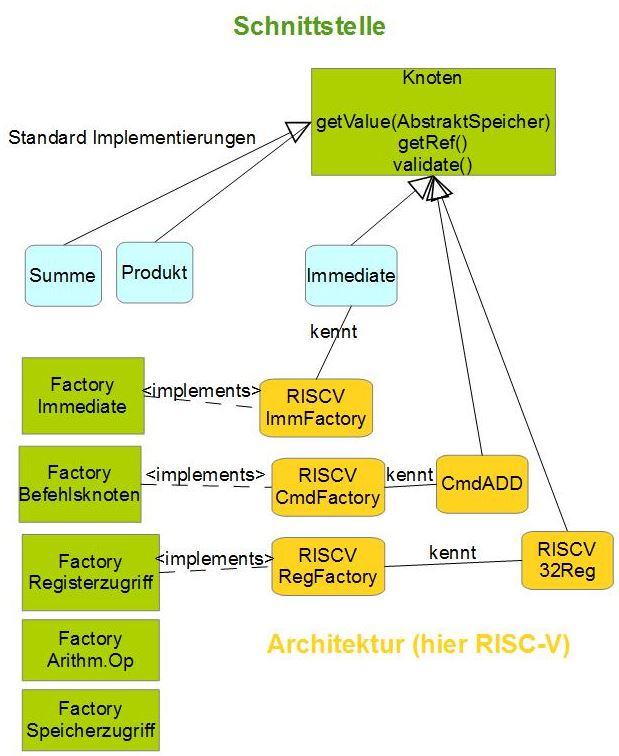
\includegraphics[scale=0.5]{../arch/figures/zeichnung}
\end{figure}

%%% Local Variables:
%%% mode: latex
%%% TeX-master: "arch"
%%% End:
